
\section{绪论}

本模板只是作为本科论文格式示例作用,为尽可能涵盖《毕业论文撰写规范》规定的内容,部分图片或表格与论文内容无关,该模板论文无研究意义,师生只做格式参考。

\subsection{哈哈嗨}

\subsection{课题研究的背景及意义}

摄像头(camera)又称为电脑相机、电脑眼等,它作为一种视频输入设备,在过去被广泛的运用于视频会议、远程医疗及实时监控等方面。近些年来,随着互联网技术的发展,网络速度的不断提高,再加上感光成像器件技术的成熟,使得摄像头得到了越来越广泛的应用。

\subsubsection{视频运动目标检测的研究现状}

视频序列中运动目标的检测与跟踪是计算机视觉和图像编码研究领域的一个重要课题,在机器人导航、智能监视系统、交通检测、医学图像处理以及视频图像压缩和传输等领域都有广泛的应用。运动目标检测就是判断视频序列中是否存在运动目标,并确定运动目标的位置。运动目标的提取主要包括运动检测以及目标提取两个步骤,其中运动检测处于整个视觉监视系统的最底层,是各种后续高级处理如目标分类,行为理解等的基础。

在近年来,随着技术的快速发展,多领域的研究都取得了显著的进展。特别是在数据处理、目标检测以及环境科学等领域,新的理论和方法不断涌现,为解决实际问题提供了有力的支持。

首先,在数据处理和导航系统的应用方面,付梦印等人深入探讨了Kalman滤波理论及其在导航系统中的应用\upcite{付梦印2003}。Kalman滤波作为一种高效的递归滤波器,通过预测和更新两个步骤,能够在存在不确定性的动态系统中估计出系统状态。这一理论在导航系统中的应用,极大地提高了系统的准确性和可靠性。

在目标检测领域,邓宇的研究为我们提供了复杂背景下运动目标检测技术的深入见解\upcite{邓宇2007}。随着计算机视觉和图像处理技术的不断发展,目标检测技术在安防、交通监控等领域的应用越来越广泛。如何在复杂的背景下准确、快速地检测出目标,成为该领域的重要研究方向。

在环境科学领域,张爱茜等人关注了氯代芳香族化合物对羊角月牙藻的毒性及QSAR分析\upcite{张爱茜2000}。这一研究不仅揭示了氯代芳香族化合物对水生生物的潜在危害,还通过QSAR(定量结构-活性关系)分析,为预测和评估这类化合物的环境风险提供了有力的工具。

此外,文献\cite{Stauffer1999}提出了自适应背景混合模型(Adaptive Background Mixture Models),为实时跟踪提供了新的解决方案。这一模型通过对背景图像进行建模和更新,能够有效地区分前景目标和背景,为视频监控、人机交互等领域的研究提供了新的思路。

综上所述,从Kalman滤波理论在导航系统中的应用,到复杂背景下的目标检测技术,再到环境科学中的毒性评估和QSAR分析,以及实时跟踪中的自适应背景混合模型,这些研究成果不仅丰富了相关领域的理论和方法,也为解决实际问题提供了有力的支持。随着技术的不断进步,相信这些领域的研究将会取得更加显著的成果。

\subsubsection{运动目标检测技术}

运动目标检测技术研究如何完成研究对象(图像序列)中感兴趣的目标区域的“准确定位”问题。

\fourthsection{帧间差分法}

三种传统的运动目标检测算法之一。帧间差分式检测相邻两帧图像之间变化的最简单、最直接的方法,它是直接比较了两帧图像对应像素点的灰度值的不同,然后通过阈值来提取序列图像中的运动区域。二值图像中为“$0$”的像素对应在前后两帧图像之间没有发生(由于运动而产生的)变化的地方,为“1”的像素对应两帧图像间发生变化的地方,这常是由目标运动而产生的。

计算得到
\begin{equation}%\label{}
Q_s = \varphi(h-z)^{3/2}F^{4/5}\beta\gamma\delta,
\end{equation}
其中,$E_s$与$E_c$分别表示基体和涂层的平均弹性模量;$\alpha_s$与$\alpha_c$分别表示基体和涂层的热膨胀系数;$\Delta T$表示喷涂前后温差;$D$与$d$分别表示基体和涂层的厚度。

{\bf 定理1.1}\upcite{付梦印2003}\quad 这里是定理内容 %想实现的效果
\begin{Theorem}[\upcite{付梦印2003}]
这里是定理内容
\end{Theorem}

将所查各值代入公式可得:
\begin{align}%\label{}
  C_0 &= \sqrt{ 2\frac{k}{k-1}RT_0^{\ast}\lt(1-\frac{1}{\prod_{T}^{m}}\rt) } \notag \\
   &= \sqrt{ 2\times \frac{1.4}{1.4-1}\times 287\times 285\times \lt( 1-\frac{1}{3^{0.286}} \rt) } \notag \\
   &= 392.9~\unit{m/s}.
\end{align}

处理过程如图\ref{fig:手部运动方向检测结构图}所示。
\begin{figure}[H]
  \centering
  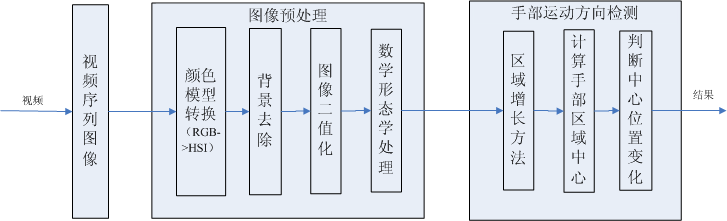
\includegraphics[width=0.8\textwidth]{fig_ch1/手部运动方向检测结构图.png}
  \caption{手部运动方向检测结构图}
  \label{fig:手部运动方向检测结构图}
\end{figure}

由图\ref{fig:手部运动方向检测结构图}可以知道,当得到一个变量的概率密度函数pdf时,熵就可以用来度量其状态的连贯性,同时,熵也是能量的一种表示。

\subsection{本章小结}

视频序列中运动目标的检测与跟踪是计算机视觉和图像编码研究领域的一个重要课题,在机器人导航、智能监视系统、交通检测、医学图像处理以及视频图像压缩和传输等领域都有广泛的应用。运动目标检测就是判断视频序列中是否存在运动目标,并确定运动目标的位置。